\documentclass[12pt,twoside]{report}
\usepackage[utf8x]{inputenc}
\usepackage{polski}
\usepackage{graphicx}
\usepackage{caption}
\usepackage{subcaption}
\usepackage[a4paper,width=150mm,top=25mm,bottom=25mm,bindingoffset=6mm]{geometry}
\usepackage{fancyhdr}
\usepackage[nottoc,numbib]{tocbibind}
\pagestyle{fancy}
\fancyhead{}
\fancyhead[RO,LE]{Sprzętowo-programowy system przetwarzania danych wektorowych}
\fancyfoot{}
\fancyfoot[LE,RO]{\thepage}
\fancyfoot[LO,CE]{Rozdział \thechapter}
\fancyfoot[CO,RE]{Tomasz Dyczek, Piotr Moczurad}
\renewcommand{\headrulewidth}{0.4pt}
\renewcommand{\footrulewidth}{0.4pt}

\title{Thesis Title}
\author{Author Name}
\date{Day Month Year}	

\begin{document}
	\begin{titlepage}
    \begin{center}
		\fontsize{17pt}{20pt}\selectfont
        \textbf{Akademia Górniczo-Hutnicza\\im. Stanisława Staszica w Krakowie}
        \rule{\textwidth}{1.5pt}\par
        \vspace{0.5cm}
        Wydział Informatyki, Elektroniki i Telekomunikacji
        
        \vspace{1.5cm}

        \includegraphics[scale=0.75]{images/agh}
 		
 		\vspace{1.5cm}
 		
 		Dokumentacja użytkownika
 		
 		\vspace{0.5cm}
	 	\textbf{Sprzętowo-programowy system\\przetwarzania danych wektorowych,\\oparty na ukladzie FPGA}
		
		Piotr Moczurad
		Tomasz Dyczek
		\vspace{1.5cm}\\
		\textbf{Opiekun}\\
		dr inż. Jacek Długopolski
		\rule{\textwidth}{1.5pt}\par
		Kraków 2015
		
        
    \end{center}
\end{titlepage}
	\tableofcontents	
	
	\chapter{Wstęp}
    \section{Struktura projektu}

Struktura projektu, a wraz z nią struktura repozytorium, odzwierciedla wyraźny podział na część software'ową (kompilator naszego języka programowania) oraz hardware'ową (koprocesor zaimplementowany na układzie FPGA). Dodatkowo, dokumentacja do projektu jest również trzymana w repozytorium, co umożliwia łatwiejszą współpracę nad jej tworzeniem i pozwala na zarządzanie jej wersjami.

Część hardware'owa, związana z FPGA, ma niemalże płaską strukturę: mamy jeden moduł główny i kilka pomniejszych komponentów, które są do niego dołączone (jako osobne części układu zaimplementowane są jego wyróżnione składowe, takie jak stos, pamięć ram czy moduł UART). Każdy z komponentów umieszczony jest w oddzielnym pliku.

Część software'owa jest w pełni autonomicznym projektem języka Haskell, budowanym systemem budowania Cabal. Narzuca to pewną strukturę plików i katalogów (w Haskellu tworzone są hierarchiczne moduły poprzez umieszczanie plików w odpowiednich ścieżkach folderów). Projekt podzielony jest na części związane z etapami kompilacji programów w naszym języku, w szczególności na dwa główne moduły: \texttt{Parser} i \texttt{CodeGen}, które z kolei podzielone są na bardziej szczegółowe submoduły. Dokładna struktura plików i katalogów została przedstawiona na rysunku \ref{fig:file_structure}.

\begin{figure}
  \begin{center}
    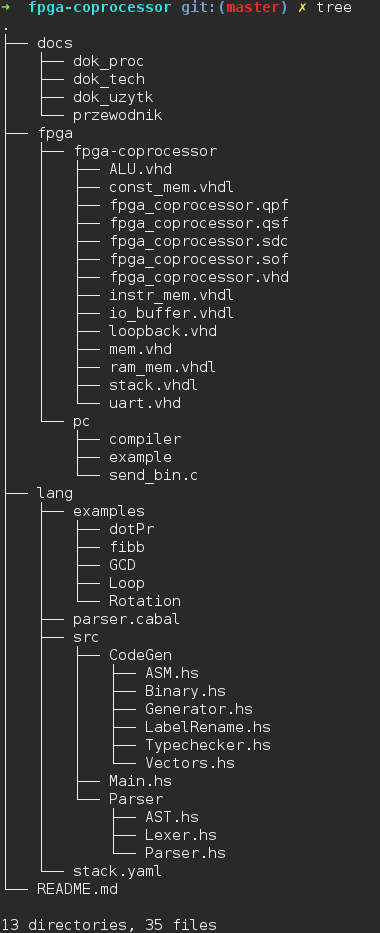
\includegraphics[scale=0.5]{images/file_structure.png}
    \caption{Struktura plików w projekcie jako wynik polecenia \texttt{tree} w systemie Linux.}
    \label{fig:file_structure}
  \end{center}
\end{figure}

\section{Porady dotyczące budowania}

Zwykły użytkownik systemu nie musi zajmować się jego budowaniem, jednak programista, pragnący rozwijać system, musi zapoznać się ze specyfiką budowania projektów języka Haskell w systemie Cabal oraz języka VHDL w środowisku Quartus.

\subsection{Haskell}
Cały projekt haskellowy mieści się w katalogu \texttt{lang}. Pierwszą rzeczą, na którą należy zwrócić uwagę jest plik \texttt{parser.cabal}. Jest to plik opisujący projekt Cabala, który służy nam m.in. do określania zależności projektu wraz z ich wersjami, dostarczania informacji o projekcie, ustawiania globalnych opcji kompilacji dla całego projektu, czy włączania rozszerzeń języka Haskell na poziomie projektu. W pliku tym możemy zdecydować, czy projekt ma być budowany jako biblioteka (\textit{library}) czy wykonywalny program (\textit{executable}). Możemy również, jak w przypadku naszego projektu, zbudować projekt na obydwa sposoby. Dla obydwu rodzajów budowania podajemy katalogi, w których kompilator ma szukać plików źródłowych (\texttt{hs-source-dirs}), opcje kompilatora (\texttt{Ghc-Options}) i zależności (\texttt{build-depends}).

Zależności są polem, na które warto zwrócić szczególną uwagę. W przeciwieństwie do systemów budowania języka Java, takich jak Maven, Cabal nie ściąga archiwów \texttt{.jar} z bibliotekami. Ściąga jedynie źródła, które potem kompiluje. Tworzy to pewne problemy z wersjami bibliotek (wyobraźmy sobie sytuację, w której biblioteka $A$ wymaga biblioteki $B$ w wersji 0.1 oraz biblioteki $C$ w wersji 0.2, a z kolei biblioteka $B$ wymaga biblioteki $C$ w wersji 0.3 --- problemy z wersjami bibliotek są powszechne przy stosowaniu Cabala), które możemy próbować obchodzić przez wymuszanie konkretnych wersji bibliotek lub ich przedziałów. W naszym projekcie jednak wybór padł na używanie wszystkich bibliotek w ich najnowszych wersjach, więc żadne wersje nie są sztucznie wymuszane. Jest to możliwe również dzięki zastosowaniu technologii \textit{sandboxów}. Zamiast instalować wszystkie biblioteki globalnie do systemu (co potencjalnie rodzi konflikty, jeśli mamy więcej niż jeden projekt), instalujemy je do osobnego środowiska umieszczonego w osobnym folderze, które możemy łatwo usunąć i odtworzyć w razie problemów.

Po zainstalowaniu projektu poleceniem \texttt{cabal install} utworzy się folder \texttt{dist}, w którym można znaleźć pliki wykonywalne i biblioteki utworzone podczas budowania. Popularną praktyką wśród programistów Haskella jest usuwanie katalogu \texttt{dist} w razie problemów z budowaniem i \texttt{.cabal-sandbox} w razie problemów z wersjami pakietów.

\subsection{FPGA}

Projekt FPGA jest utworzony w środowisku Quartus II firmy Altera, które automatyzuje budowanie projektu przez dostarczenie zintegrowanego środowiska do projektowania i syntezy układów. Kompilacja odbywa się za pomocą graficznego interfejsu i nie wymaga szczegółowego opisywania. W razie problemów z kompilacją Altera dostarcza obszerną dokumentację do środowiska Quartus. Ważnym plikiem jest \texttt{fpga\_coprocessor.qsf}, który zawiera przypisania pinów (\textit{pin assignments}) dla projektu. W przypadku budowania projektu dla innej płytki, niż Altera De0-Nano, należy zmienić plik tak, by nazwy pinów odpowiadały tym, które faktycznie są dostępne na płytce. Jest to o tyle istotne, że w przypadku rozszerzania układu może zajść konieczność użycia większej płytki (z większą ilością elementów logicznych i szybszym wejściem-wyjściem).

\subsection{Komunikacja}

Aby skompilować prosty program do obsługi komunikacji z koprocesorem, który można znaleźć w katalogu \texttt{fpga/pc} wystarczy zwyczajny kompilator języka C. Przy tworzeniu projektu wykorzystano kompilator GCC w wersji 5.1, choć każdy kompilator obsługujący standard C99 wystarczy do skompilowania programu. Przykładowe polecenie to: \texttt{gcc -o sender sender.c}. Dodatkowo, komunikacja odbywa się przez port szeregowy, więc trzeba zadbać, by urządzenie w systemie, jako które widoczny jest nasz port, było faktycznie rozpoznawane przez system jako port szeregowy. Służy temu polecenie \texttt{setserial}, dostępne w systemach linuksowych po zainstalowaniu pakietu o tej samej nazwie. Przykładowo, używając systemu Fedora 22 musimy wydać polecenie: \texttt{sudo dnf install setserial \&\& sudo setserial -g /dev/ttyUSB0}. W powyższych instrukcjach bazujemy na założeniu, że do komunikacji używana jest przejściówka USB-UART. Jeśli do rozwoju systemu zostanie użyty inny sposób podłączenia (np. bezpośrednio do pinów GPIO na urządzeniach typu Arduino bądź Raspberry Pi), nazwa urządzenia może ulec zmianie.


    \chapter{Opis modułów}
    Podczas implementacji systemu udało się większość stawianych mu wymagań funkcjonalnych i niefunkcjonalnych. Specyfika tematu, a w szczególności jego otwartość na rozwój i skalowanie powoduje, że każdą ze zrealizowanych funkcjonalności można jeszcze dalej rozwijać oraz dodawać nowe praktycznie bez ograniczeń. Mówiąc najogólniej: spełnione zostało podstawowe kryterium, o którym wspomniano w poprzednim rozdziale, tj. otrzymaliśmy w pełni działający system, który potwierdza naszą tezę i wykonuje zadanie, jakie mu powierzono.

\section{Zarys wymagań}
Pierwszym i podstawowym wymaganiem stawianym systemowi jest sprawne i bezbłędne przetwarzanie danych. Potrzeba szybkości nie podlega dyskusji -- projektując systemy przetwarzania danych jest to zawsze jednym z podstawowych kryteriów oceny systemu. Bezbłędność jest kolejnym niezwykle ważnym kryterium: podczas dość skomplikowanej ścieżki, jaką pokonują dane w naszym programie jest wiele miejsc, w których dane mogą ulec przekłamaniu lub może wkraść się do nich błąd.

Tak więc po pierwsze potrzebujemy kompilatora, który produkuje poprawne programy. Niezwykle łatwo przy budowie języka przeoczyć pewne własności, które ujawniają się dopiero przy pewnych szczególnych sytuacjach (jak na przykład pętla o zerowej ilości iteracji). Przez poprawność programów rozumiemy nie tylko poprawność logiczną kodu maszynowego, ale również odfiltrowanie niepoprawnych programów użytkownika. Po drugie, transmisja danych musi być niezawodna. Przy niskopoziomowym przesyłaniu danych przez port szeregowy łatwo może dojść do przekłamania niektórych bitów i w efekcie do zepsucia całego wysyłanego do koprocesora programu. Aby tego uniknąć, należy zadbać o właściwą obsługę portu od strony oprogramowania, układu FPGA, jak i sprzętu użytego do połączenia całego systemu. Kolejnym elementem warunkującym poprawność działania systemu jest właściwa implementacja układu na FPGA, gdzie łatwo o subtelne pomyłki, jak na przykład za mała liczba cykli przeznaczanych na odczyt z pamięci.

Możemy zatem wyróżnić w naszym systemie wymagania funkcjonalne:
\begin{itemize}
  \item stworzenie języka programowania, wspierającego m.in. następujące operacje:
  \begin{itemize}
    \item deklaracje i przypisania zmiennych
    \item instrukcje warunkowe
    \item pętle
    \item kontrolę typów
    \item operacje arytmetyczne na wektorach
  \end{itemize}
  \item kompilacja programów w wyżej opisanym języku do postaci binarnej
  \item przesyłanie programów do procesora na układzie FPGA
  \item odbieranie wyników z procesora
  \item wykonanie programu na procesorze (operacje na krótkich wektorach powinny być atomowe i wykonywać się w stałej, niewielkiej liczbie cykli)
\end{itemize}

Dodatkowo, możemy mówić o (wspomnianych wyżej) wymaganiach niefunkcjonalnych:
\begin{itemize}
  \item ,,wysokopoziomowość'' języka -- użytkownik nie powinien pisać ręcznie typowych działań na wektorach
  \item wygoda przetwarzania danych wektorowych
  \item wydajność całego systemu
  \item niezawodność i brak błędów (istone zwłaszcza przy implementacji komunikacji między komputerem a układem FPGA)
\end{itemize}

\section{Zrealizowane funkcjonalności}
Wyniki przeprowadzanych testów wskazują, że system spełnia powyższe wymagania. Wydajność systemu gwarantowana jest przez równoległość przetwarzania danych po stronie koprocesora, oraz odpowiedni dobór technologii i przemyślany program po stronie kompilatora (użyto języka Haskell, który świetnie nadaje się do tworzenia kompilatorów, a dodatkowo posiada niezwykle dopracowany, optymalizujący kompilator GHC).


Funkjonalności dostarczane przez system to:
\begin{itemize}
  \item kompilacja programów napisanych w dedykowanym języku programowania, ukierunkowanym na przetwarzanie danych wektorowych. Język wspiera natywnie operacje arytmetyczne na wektorach, takie jak: dodawanie, odejmowanie, mnożenie (skalarne), dzielenie (element-przez-element) oraz posiada mechanizm statycznego sprawdzania długości wektorów. Kompilacja przebiega kilkuetapowo i składa się między innymi z fazy parsowania, sprawdzania typów (typecheckingu), generacji kodu assemblera i binaryzacji.
  \item własny język assembler, przystosowany do architektury koprocesora, uwzględniający wektorową naturę języka.
  \item wykonywanie programów na koprocesorze, zaimplementowanym na układzie FPGA. Koprocesor ma architekturę wektorową, co oznacza, że wektorowe operacje na wektorach stałej długości są wykonywane w jednym cyklu zegara, a większe wektory są rozbijane na mniejsze -- takie, które procesor potrafi obsłużyć w jednym cyklu.
  \item przesyłanie skompilowanych programów w postaci binarnej z komputera na koprocesor i z powrotem za pomocą portu UART (transmisja szeregowa).
\end{itemize}


	  \chapter{Uwagi końcowe}
    \section{Section Title}
Lorem ipsum dolor sit amet, consectetur adipisicing elit, sed do eiusmod tempor incididunt ut labore et dolore magna aliqua. Ut enim ad minim veniam, quis nostrud exercitation ullamco laboris nisi ut aliquip ex ea commodo consequat. Duis aute irure dolor in reprehenderit in voluptate velit esse cillum dolore eu fugiat nulla pariatur. Excepteur sint occaecat cupidatat non proident, sunt in culpa qui officia deserunt mollit anim id est laborum.

Lorem ipsum dolor sit amet, consectetur adipisicing elit, sed do eiusmod tempor incididunt ut labore et dolore magna aliqua. Ut enim ad minim veniam, quis nostrud exercitation ullamco laboris nisi ut aliquip ex ea commodo consequat. Duis aute irure dolor in reprehenderit in voluptate velit esse cillum dolore eu fugiat nulla pariatur. Excepteur sint occaecat cupidatat non proident, sunt in culpa qui officia deserunt mollit anim id est laborum.

Lorem ipsum dolor sit amet, consectetur adipisicing elit, sed do eiusmod tempor incididunt ut labore et dolore magna aliqua. Ut enim ad minim veniam, quis nostrud exercitation ullamco laboris nisi ut aliquip ex ea commodo consequat. Duis aute irure dolor in reprehenderit in voluptate velit esse cillum dolore eu fugiat nulla pariatur. Excepteur sint occaecat cupidatat non proident, sunt in culpa qui officia deserunt mollit anim id est laborum.

Lorem ipsum dolor sit amet, consectetur adipisicing elit, sed do eiusmod tempor incididunt ut labore et dolore magna aliqua. Ut enim ad minim veniam, quis nostrud exercitation ullamco laboris nisi ut aliquip ex ea commodo consequat. Duis aute irure dolor in reprehenderit in voluptate velit esse cillum dolore eu fugiat nulla pariatur. Excepteur sint occaecat cupidatat non proident, sunt in culpa qui officia deserunt mollit anim id est laborum.

Lorem ipsum dolor sit amet, consectetur adipisicing elit, sed do eiusmod tempor incididunt ut labore et dolore magna aliqua. Ut enim ad minim veniam, quis nostrud exercitation ullamco laboris nisi ut aliquip ex ea commodo consequat. Duis aute irure dolor in reprehenderit in voluptate velit esse cillum dolore eu fugiat nulla pariatur. Excepteur sint occaecat cupidatat non proident, sunt in culpa qui officia deserunt mollit anim id est laborum.

\section{Section Title}
Lorem ipsum dolor sit amet, consectetur adipisicing elit, sed do eiusmod tempor incididunt ut labore et dolore magna aliqua. Ut enim ad minim veniam, quis nostrud exercitation ullamco laboris nisi ut aliquip ex ea commodo consequat. Duis aute irure dolor in reprehenderit in voluptate velit esse cillum dolore eu fugiat nulla pariatur see \ref{fig:x cubed graph}. Excepteur sint occaecat cupidatat non proident, sunt in culpa qui officia deserunt mollit anim id est laborum.


    
    
	%Bibliografia
    \begin{thebibliography}{99}
\bibitem{pa} Miran Lipovača:
\emph{Learn You a Haskell for Great Good!},
Nostarch, April 2011

\bibitem{pa} Bryan O'Sullivan, John Goerzen, Donald Bruce Stewart:
\emph{Real World Haskell},
O'Reilly Media, 2008

\bibitem{pa} Alfred V. Aho, Monica S. Lam, Ravi Sethi, Jeffrey D. Ullman:
\emph{Compilers: Principles, Techniques, and Tools (2nd Edition)},
Addison Wesley; 2nd edition (September 10, 2006)


\bibitem{pa} Philip Coopman, Jr.:
\emph{Stack Computers, the new wave},
Mountain View Press ('89)

\bibitem{pa}
\emph{Quartus II Introduction Using VHDL Design},
Altera, May 2011

\bibitem{pa}
\emph{DE0-Nano, User manual},
Altera, May 2013


\bibitem{pa} Peter Yiannacouras:
\emph{FPGA-Based Soft Vector Processors},
University of Toronto, 2009

\bibitem{pa} KeyStone Architecture:
\emph{Universal Asynchronous Receiver/Transmitter (UART)},
Texas Instruments, November 2010

\bibitem{pa}Peter A Bennet:
\emph{RS232 UART (VHDL)}
http://bytebash.com/2011/10/rs232-uart-vhdl/

\end{thebibliography}

\end{document}
